\documentclass[tikz]{standalone}
\usepackage{amssymb,dsfont}
\usepackage{color}
\usetikzlibrary{arrows}
% Sets
\newcommand{\CC}{\mathbb{C}}        % Complex numbers
\newcommand{\NN}{\mathbb{N}}        % Natural numbers
\newcommand{\RR}{\mathbb{R}}        % Real numbers
\newcommand{\ZZ}{\mathbb{Z}}        % Relative integers
% Groups
\newcommand{\SO}{\mathrm{SO}}       % Special orthogonal group
\newcommand{\OO}{\mathrm{O}}        % Orthogonal group
\newcommand{\SU}{\mathrm{SU}}       % Special unitary group
\newcommand{\1}{\mathds{1}}		    % trivial group
\newcommand{\DD}{\mathbb{D}}        % Dihedral group
\newcommand{\octa}{\mathbb{O}}      % Cubic (octahedral) group
\newcommand{\ico}{\mathbb{I}}       % Icosahedral group
\newcommand{\tetra}{\mathbb{T}}     % tetrahedral group
\begin{document}
	
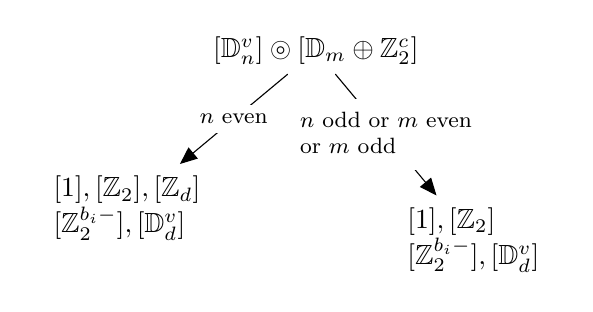
\begin{tikzpicture}[scale=0.8,line cap=round,line join=round,>=triangle 45,x=1.0cm,y=1.0cm]
  \node (root) at (0,0) {$[\DD_n^v]\circledcirc [\DD_m\oplus \ZZ_2^c]$};

  \node (Bas1) at (-3,-2.5) {\begin{tabular}{l} $[\1],[\ZZ_2],[\ZZ_d]$ \\$[\ZZ_2^{b_i-}],[\DD_d^v]$ \end{tabular}};
  \node (Bas2) at (2.5,-3)   {\begin{tabular}{l} $[\1],[\ZZ_2]$ \\$[\ZZ_2^{b_i-}],[\DD_d^v]$ \end{tabular}};
  \draw [->](root) -- (Bas1) node [midway,fill=white] {{\footnotesize $n$ even }};
  \draw [->](root) -- (Bas2) node [midway,fill=white] {{\footnotesize  \begin{tabular}{l} $n$ odd or $m$ even \\ or $m$ odd \end{tabular}}};
\end{tikzpicture}
% Further ’tikzpicture’ environments are possible which will create further pages.
\end{document} 